\chapter{Architecture and System Design}
\label{chap:architecture}

This chapter aims to explore the architecture and design of the CardioSync framework, building upon the problem statement from Chapter \ref{chp:introduction}.
\vspace{1\baselineskip}

\noindent In response to those challenges, this chapter outline the architectural evolution from FreeBie to CardioSync, highlighting the transformative integration of the framework. Also this chapter, we provide a thorough analysis of the proposed architecture, focusing on key components, interactions, and overall design concepts.
\vspace{1\baselineskip}

\begin{figure}[t]
    \centering
    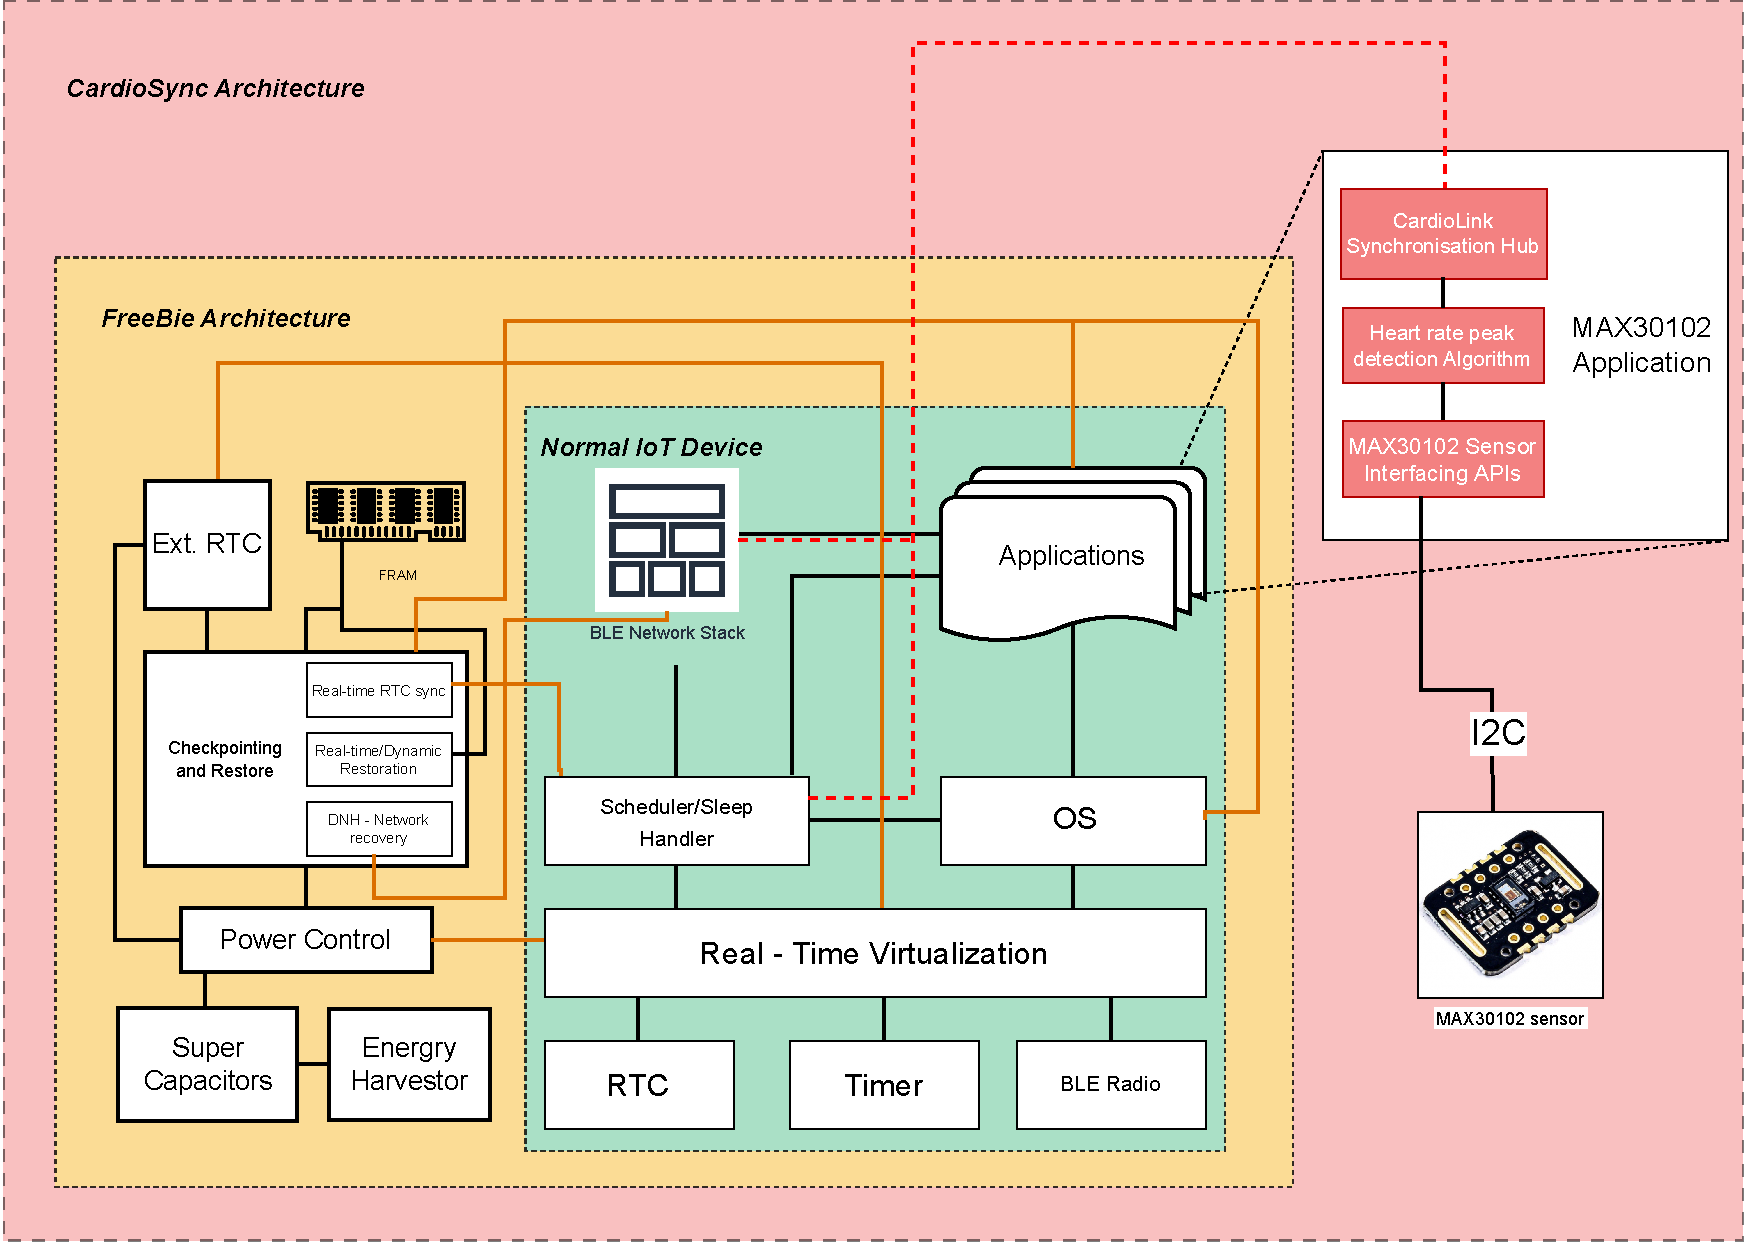
\includegraphics[width=\linewidth]{chapters/Architecture/architecture.pdf}
    \caption{High Level Architecture of the CardioSync framework.}
    \label{fig:architecture}
\end{figure}

\noindent Furthermore, to aid in understanding the conceptual landscape, \autoref{fig:architecture} illustrates the high-level architecture of the CardioSync framework within the existing FreeBie model.

\section{CardioSync Framework}
The architecture of FreeBie, as described in Section \ref{sec:freebie_architecture}, employs periodic advertisement for BLE connection establishment in an end device. However, this approach can lead to asynchrony between the end device's periodic advertisement and the BLE host's scan, resulting in a hindrance to establishing a successful connection when both are intermittently-powered.
\vspace{1\baselineskip}

\noindent Addressing this limitation, the CardioSync framework augments over the FreeBie architecture to orchestrate BLE connection setup events in synchronisation with the host's events through the utilisation of a shared external signal. By doing so, CardioSync enables bidirectional intermittent operation for FreeBie. Moreover, the final CardioSync architecture collaborates seamlessly with FreeBie for scheduling a wake-up and sleep cycle that aligns with synchronised connection setups and adapts to the dynamic power availability of intermittently-powered devices.
\vspace{3\baselineskip}
\begin{figure}[t]
    \begin{subfigure}{1\linewidth}
        \centering
        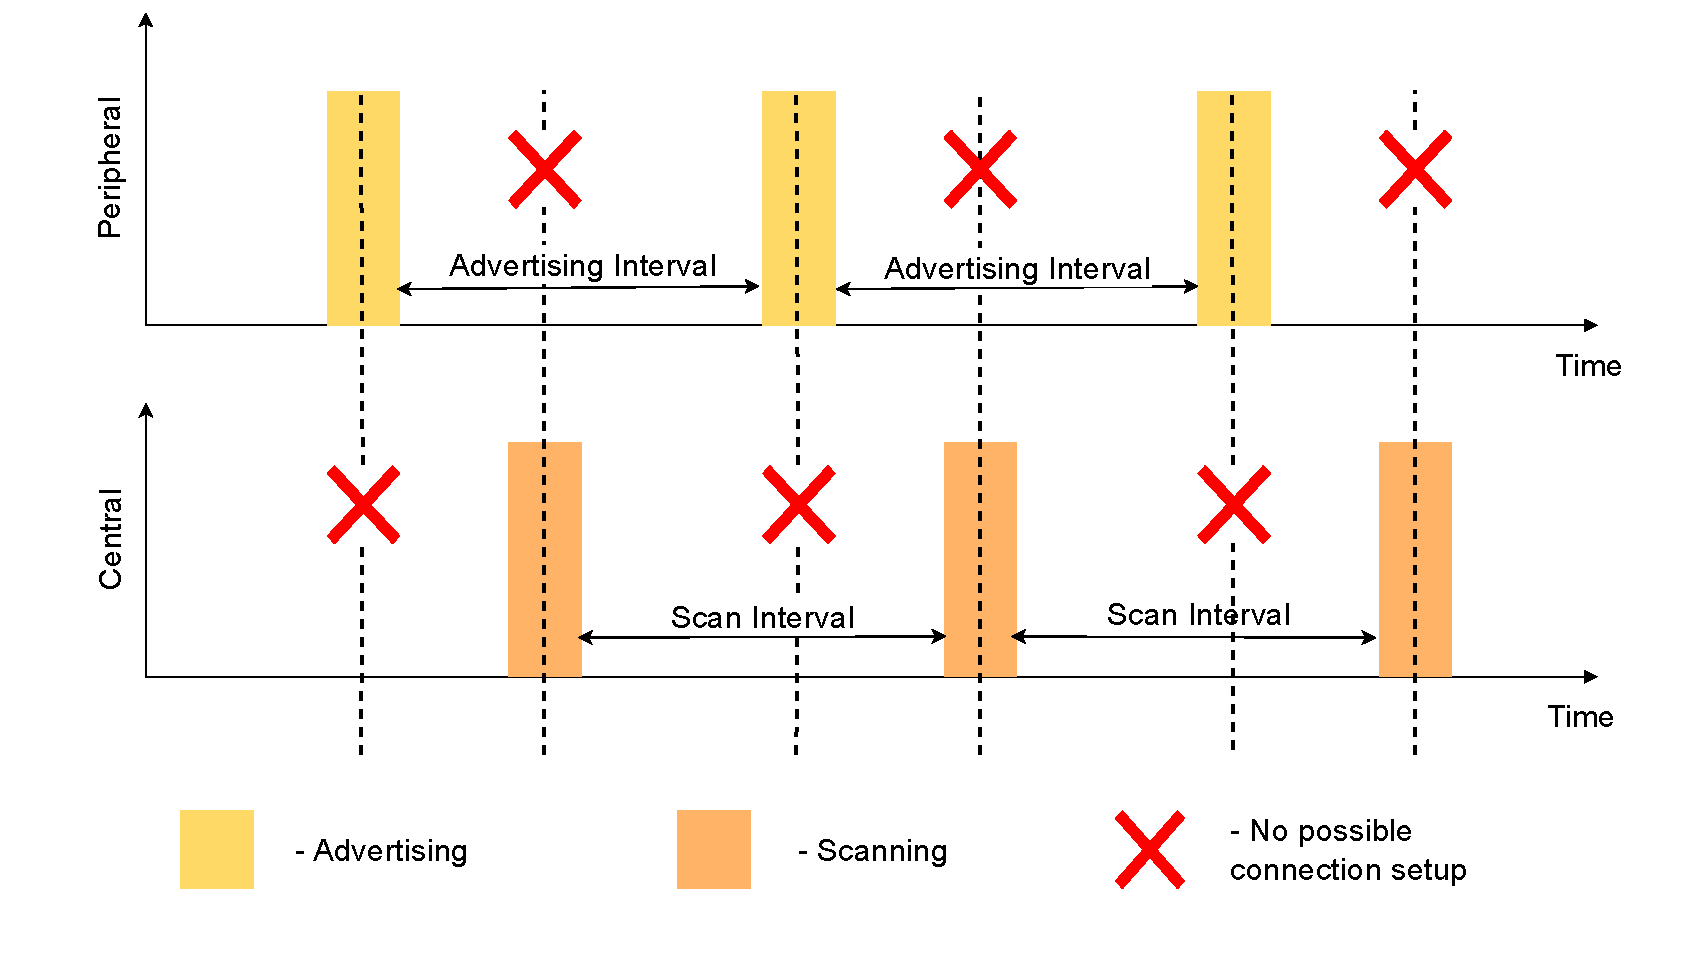
\includegraphics[width=\linewidth]{chapters/Architecture/Freebie_concept.pdf}
        \subcaption{Conceptual diagram illustrating failed asynchronous periodic connection setup attempts in a FreeBie system.}
        \label{fig:concept_freebie}
        \vspace{3\baselineskip}
    \end{subfigure}
    \begin{subfigure}{1\linewidth}
        \centering
        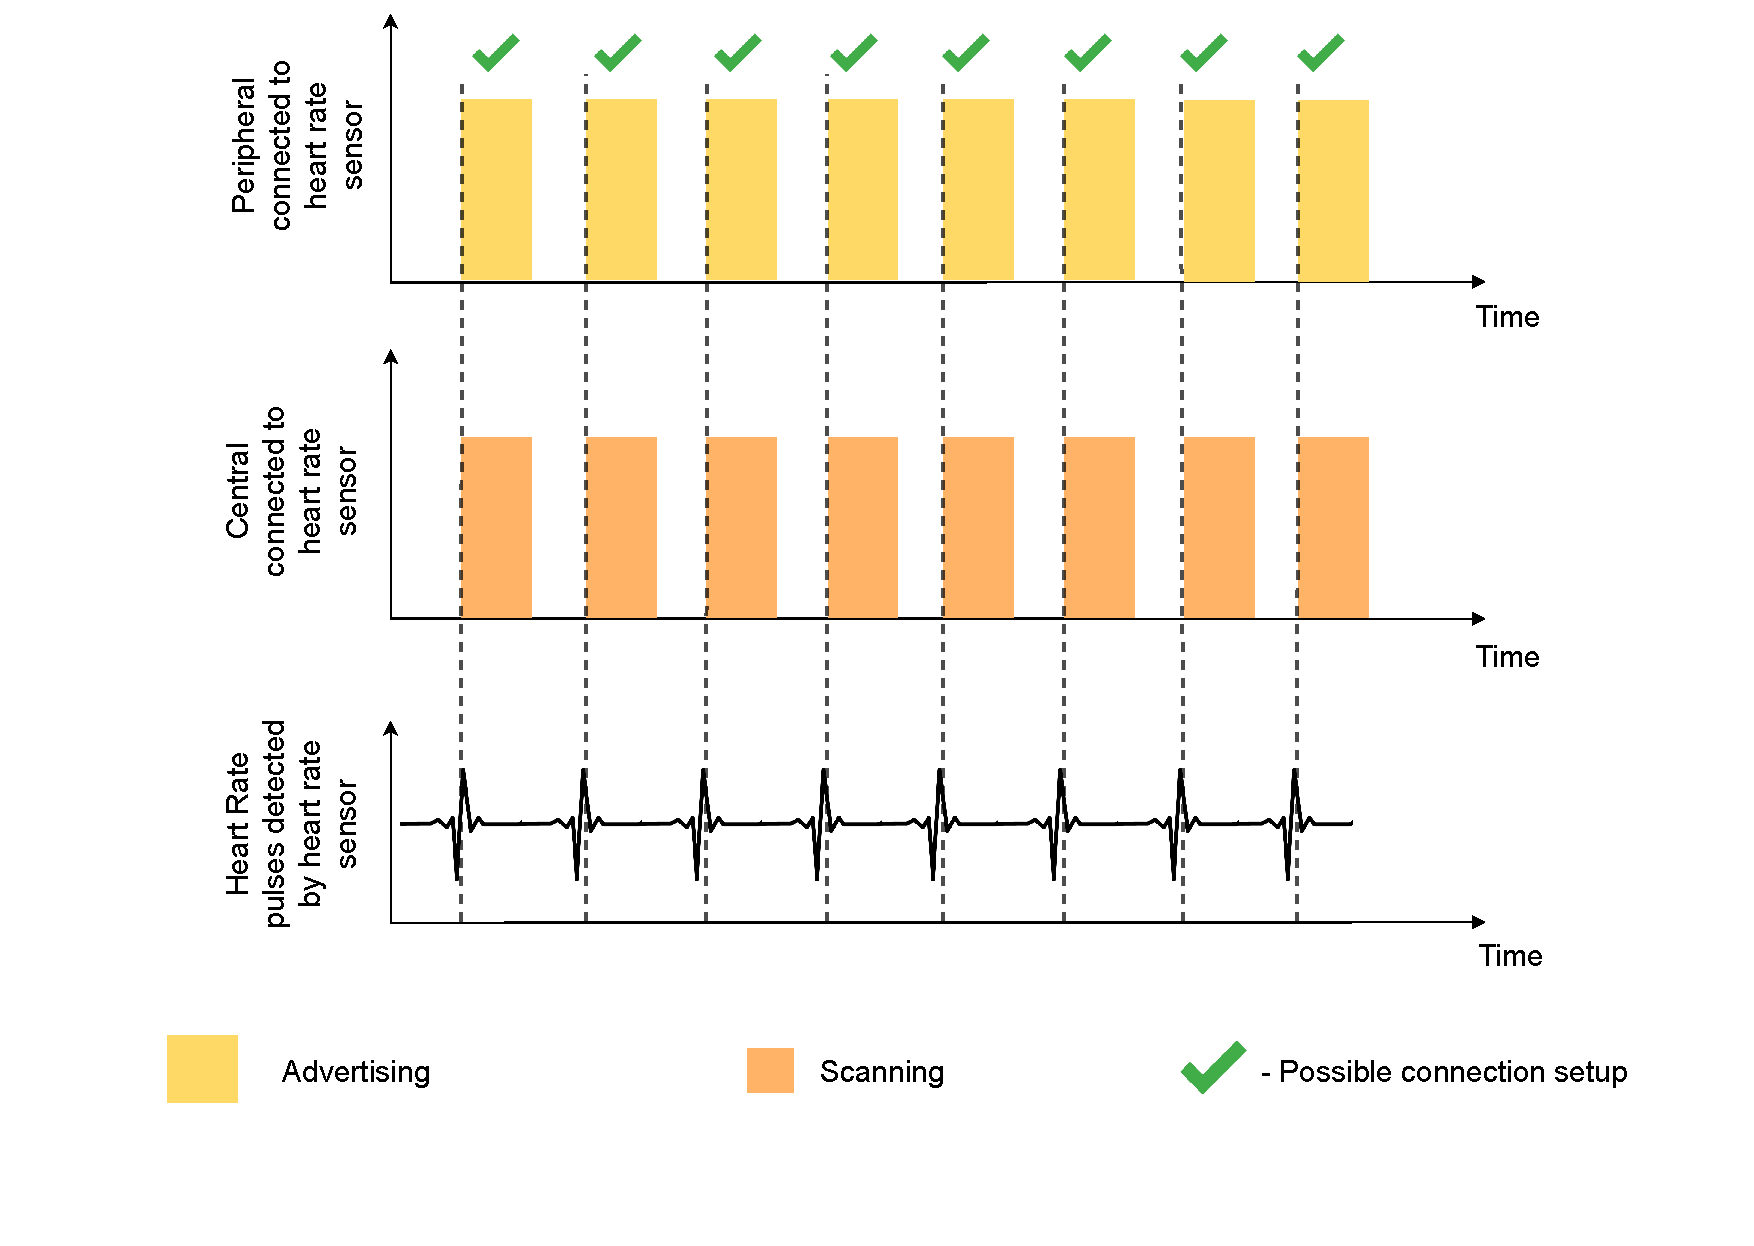
\includegraphics[width=\linewidth]{chapters/Architecture/CardioSync_concept.pdf}
        \caption{Conceptual diagram illustrating possible synchronised connection setup attempts in a CardioSync system. Advertising of peripheral and scanning of central is synchronised by heart rate pulses detected by heart rate sensor connected to the devices.}
        \label{fig:concept_cardiosync}
    \end{subfigure}
    \caption{}
    \label{fig:freebie_vs_cardiosync}
\end{figure}
\clearpage

\noindent Figure \ref{fig:concept_freebie} highlights the difficulty encountered in establishing a connection between intermittent devices using the FreeBie architecture. Additionally Figure 
\ref{fig:concept_cardiosync} showcases the planned approach used by CardioSync to address this obstacle via the utilisation of external clock as heart rate pulses.
\vspace{1\baselineskip}

\noindent The CardioSync framework is structured around the novel heart rate peak detection algorithm that detects peaks effectively based on raw data from a low power heart rate sensor. This algorithm serves as the basis for initiating synchronised connection events and also establishing synchronisation points which are strategically defined moments in time based on heart rate.
\vspace{1\baselineskip}

\noindent The CardioSync framework integrates into the FreeBie architecture, leveraging key components that contribute to the framework's enhanced functionality:

\begin{itemize}
    \item \textbf{Low-Power Heart Rate Sensor:}
    The foundation of the CardioSync framework lies in a carefully selected low-power heart rate sensor. This sensor efficiently captures raw heart rate data, providing the essential input for synchronisation and connection setup activities.

    \item \textbf{CardioSync Real-Time Application:} This extension to the FreeBie architecture introduces the CardioSync module, encompassing several subcomponents responsible for different aspects of the synchronisation process.
    \begin{itemize}
        \item \textbf{Sensor Data Collector:} This subcomponent interfaces with the low-power heart rate sensor, collecting accurate heart rate data. It ensures seamless data acquisition and serves as the initial step in the synchronisation process. It houses the sensor interfacing functionality along with data pre-processing as required for the algorithm.
        
        \item \textbf{Heart Rate Peak Detection Algorithm:} At the heart of the CardioSync framework, this subcomponent processes the heart rate data collected by the sensor data collector. It intelligently identifies heart rate peaks, which serve as synchronisation triggers for connection setup events and establish synchronisation points. These synchronised trigger points are coupled with active sensor reads hence adhering to "Read and Synchronise" phase of CardioSync framework to establish a connection.
        
        \item \textbf{Connection Control:} This subcomponent manages the setup of BLE connections via strategic scheduling. It leverages cues from the heart rate peak detection algorithm to time connection setup events, aligning them with heart rate interval. This integration utilises the Checkpointing and Restore component in the FreeBie architecture by effectively using Timers. Thereby ensuring the energy-efficient communication through "Sleep and Synchronise" phase of CardioSync framework.
    \end{itemize}
\end{itemize}
\noindent These components collectively empower the CardioSync framework to synchronise communication activities with heart rate patterns, enabling bidirectional intermittent operation and efficient utilisation of intermittently-powered devices.

\section{High-Level Operation Flow}
% \begin{algorithm}[t]
%     \caption{High-Level CardioSync Operation}
%     \label{alg:architectureflow}
%     \begin{algorithmic}[1]
%         \State \textbf{Sensor Data Acquisition:}
%         \State \qquad Gather sensor data through dedicated interfaces.
% \item[] 
%         \State \textbf{Heart Rate Peak Detection:}
%         \State \qquad Detect heart rate peaks
%         \State \qquad Calculate the average time interval between detected peaks.
%         \State \qquad Define interval as the temporal spacing between synchronisation points.
% \item[]
%         \State \textbf{Connection Control:}
%         \State \qquad Upon detecting a heart rate peak:
%         \State \qquad \qquad Schedule BLE advertising or scanning tasks.
%         \State \qquad \qquad Utilise timers to initiate connection at each synchronisation points.
% \item[] 
%         \State \textbf{Checkpointing and Restore:}\Comment{\textit{Operating within FreeBie architecture}}:
%         \State \qquad Monitor for inactivity between synchronisation points.
%         \State \qquad If pending tasks (e.g., next connection setup event) are scheduled:
%         \State \qquad \qquad Engage checkpointing the context
%         \State \qquad \qquad Halt MCU's operation and sleep till next pending task
%         \State \qquad \qquad Reactivate MCU and restore the context for pending task.
%     \end{algorithmic}
% \end{algorithm}

\noindent The CardioSync framework operates through a systematic sequence of steps in integration with FreeBie architecture for establishing a connection

\begin{enumerate}
    \item \textbf{Sensor Data Acquisition:} The process begins with the gathering of heart rate sensor data through dedicated interfaces.
    
    \item \textbf{Heart Rate Peak Detection:} The acquired sensor data is processed by the heart rate peak detection algorithm. This algorithm identifies distinctive peaks that correspond to heart rate activity, simultaneously calculating the average time interval between these peaks. This interval defines the temporal spacing between synchronisation points.
    
    \item \textbf{Connection Control:} Upon detecting a heart rate peak, the Connection Control component springs into action. It orchestrates the scheduling of BLE advertising or scanning events. Additionally, it optimally utilises the timers within the FreeBie architecture to initiate connection setup events that is precisely aligned with established synchronisation points.

    \item \textbf{Time-Deterministic Checkpointing and Restore:} Operating within the FreeBie architecture, this module monitors periods of system inactivity, which in our case align with the intervals between synchronisation points set by the Connection Control component. It employs checkpointing to briefly pause the MCU's operations, reactivating only when there are pending tasks, such as the next connection setup event at next synchronisation point.

\end{enumerate}